\clearpage

\subsection{Opaque with 1+1 Protection}\label{heuristic_Opaque_Protection}
\begin{tcolorbox}	
\begin{tabular}{p{2.75cm} p{0.2cm} p{10.5cm}} 	
\textbf{Student Name}  &:& Tiago Esteves    (October 03, 2017 - )\\
\textbf{Goal}          &:& Implement the heuristic model for the opaque transport mode with 1 plus 1 protection.
\end{tabular}
\end{tcolorbox}

\subsubsection{Model description}

The impact of failure in WDM (Wavelength Division Multiplexing) networks is caused by extremely high volume of traffic carried. In a high speed network like the WDM, a failure of a network element may cause failure of various optical channels that leads to large data and revenue losses, which can interrupt communication services.

In this protection scheme, the primary and backup path carry the traffic end-to-end, i.e., there is a need to have a backup path (the unaffected path) in case of a network failure. Then, the receiver will decide which one of the two incoming traffic it is going to pick, if the primary or the backup path.

Although it is the fastest protection scheme, it is also the most expensive, because it normally uses more than the double of the capacity for the primary path. This happens because the backup path is typically longer than the primary.

For this protection model, after the creation of the matrices and the network topology, it is necessary to apply the routing and grooming algorithms created. For the "Logical Topology" algorithm, the user must insert "Opaque" in the "logicalTopology" value and for the "Grooming" algorithm, the user must insert "yes" in the parameter value "protection".

At the end, the "Cost Report" algorithm will be applied to obtain the best CAPEX result for the network in question.

\subsubsection{Result description}

We already have all the necessary formulas to obtain the CAPEX value for the reference network \ref{Reference_Network_Topology}. As described in the subsection of network traffic \ref{Reference_Network_Traffic}, we have three values of network traffic (low, medium and high traffic), so we have to obtain three different CAPEX.\\

\textbf{Low Traffic Scenario:}\\

Following all the steps mentioned in the previous subsection and using all the data referring to this scenario, the obtained result can be consulted in the following figure \ref{Low_Network_Cost_Protec_Opaque}.

\begin{figure}[h!]
\centering
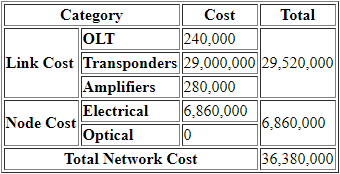
\includegraphics[width=10cm]{sdf/heuristic/figures/Low_Network_Cost_Protec_Opaque}
\caption{The low traffic network cost with 1+1 protection using Net2Plan.}
\label{Low_Network_Cost_Protec_Opaque}
\end{figure}

\begin{figure}[h!]
\centering
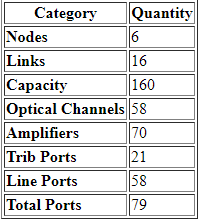
\includegraphics[width=5cm]{sdf/heuristic/figures/Low_Network_Info_Protec_Opaque}
\caption{The low traffic network info with 1+1 protection using Net2Plan.}
\label{Low_Network_Info_Protec_Opaque}
\end{figure}

\newpage
\textbf{Medium Traffic Scenario:}\\

Following all the steps mentioned in the previous subsection and using all the data referring to this scenario, the obtained result can be consulted in the following figure \ref{Medium_Network_Cost_Protec_Opaque}.

\begin{figure}[h!]
\centering
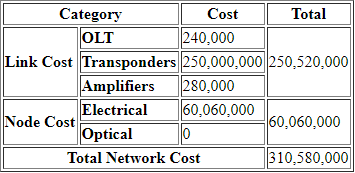
\includegraphics[width=10cm]{sdf/heuristic/figures/Medium_Network_Cost_Protec_Opaque}
\caption{The medium traffic network cost with 1+1 protection using Net2Plan.}
\label{Medium_Network_Cost_Protec_Opaque}
\end{figure}

\begin{figure}[h!]
\centering
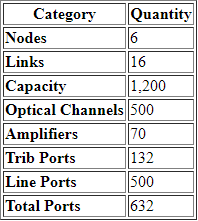
\includegraphics[width=5cm]{sdf/heuristic/figures/Medium_Network_Info_Protec_Opaque}
\caption{The medium traffic network info with 1+1 protection using Net2Plan.}
\label{Medium_Network_Info_Protec_Opaque}
\end{figure}

\newpage
\textbf{High Traffic Scenario:}\\

Following all the steps mentioned in the previous subsection and using all the data referring to this scenario, the obtained result can be consulted in the following figure \ref{High_Network_Cost_Protec_Opaque}.

\begin{figure}[h!]
\centering
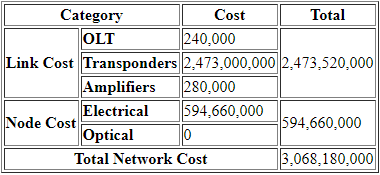
\includegraphics[width=10cm]{sdf/heuristic/figures/High_Network_Cost_Protec_Opaque}
\caption{The hight traffic network cost with 1+1 protection using Net2Plan.}
\label{High_Network_Cost_Protec_Opaque}
\end{figure}

\begin{figure}[h!]
\centering
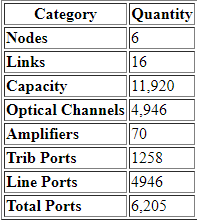
\includegraphics[width=5cm]{sdf/heuristic/figures/High_Network_Info_Protec_Opaque}
\caption{The high traffic network info with 1+1 protection using Net2Plan.}
\label{High_Network_Info_Protec_Opaque}
\end{figure}
